%!TEX root = main-doc.tex
%
% File: methodology.tex
%
% Date: ? 
%
% Description:
%   
%
%
\chapter{Methodology} \label{chap:methodology}
\vspace{-1cm}
Based on the literature review in Chapter \ref{chap:background}, it is evident that the extendibility of multidimensional sparse arrays is an incredibly important topic that has been overlooked, specifically with regards to data warehousing and OLAP. In order to make a contribution to this field, an extendible multidimensional sparse array model must be developed, implemented and evaluated. This chapter presents the proposed model design and experimental procedures for the research study.

Consider a 2D array $A[N_i][N_j]$ with bounds $N_i N_j$. An element denoted by $a<i,j>$ or equivalently $a_{ij}$ gives the value stored in location $<i,j>$ of the array. The locations $<i,j>$ are mapped into a set of linear locations $I[0, ..., M-1]$ where $M=N_i X N_j$. A mapping function $f(i,j)$, gives the location $I[l]$ where $a<i,j>$ is stored. An example of such a mapping function is the conventional row-major order allocation where $l=f(i,j)$ and $f(i,j)$ is defined as $f(i,j) = iN_j+j$.

%%%%%%%%%%%%%%%%%%%%%%%%%%%%%%%%%%%%%%%%%%%%%%%%%%%%%%%%%%%%%%%%%%%%%%%%%%%%%%%%
\section{Extendible Multi-Dimensional Sparse Arrays}
In Chapters \ref{chap:introduction} and \ref{chap:background} it was noted that a multidimensional representation of data in data warehousing provides a good conceptual view of the data to the user, as well as providing a storage scheme for efficient processing. It was also noted that these multidimensional representations need to expand dynamically as the data in a data warehouse grows dynamically. Data warehouses predominantly generate sparse arrays. Indexing a 2D dense array using its column and row indexes (i.e. $<i,j>$ = value) is fine for dense arrays, however when it comes to sparse arrays this technique is cumbersome and wastes storage space. In sparse arrays some elements are missing thus we need to store them in a compressed format to ensure that they can be use efficiently.

In order to represent a data warehouse in a multidimensional space a formula needs to be defined to increase the dimensionality of the storage scheme without changing the mapping function $f(i,j)$. As sparse data warehouses consist of large quantities of information with few non-zero elements, an efficient storage scheme that represents these non-zero elements must be chosen. Furthermore a method for extendibility of the multi-dimensional sparse array representation must be chosen.

%%%%%%%%%%%%%%%%%%%%%%%%%%%%%%%%%%%%%%%%%%%%%%%%%%%%%%%%%%%%%%%%%%%%%%%%%%%%%%%%
\section{Multi-Dimensional Sparse Array Representation}
In order to improve the storage efficiency of multi-dimensional sparse arrays, a good storage scheme must be chosen. A comparison of the different sparse array storage techniques detailed in Section \ref{chap:background} is carried out.

\subsection{Matrix Market Format}

Given the example data warehouse in Figure \ref{fig:exampleMatrix} one can use a simple matrix market format (otherwise known as a relational table) to represent the information as shown in Table \ref{tab:matrixmarket}. When using matrix market format the row index and the column index of each non-zero element is stored along with its value in a 2D array.

 \begin{figure}[H]
	\centering
	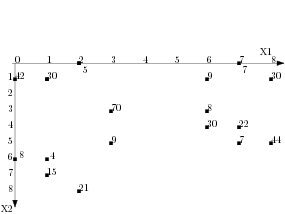
\includegraphics[width=0.7\linewidth]{exampleMatrix}
	\caption{A Sparse 2D Array}
	\label{fig:exampleMatrix}
\end{figure}

 \begin{table}[H]
	\caption{Matrix Market Format\label{tab:matrixmarket}}
	\begin{center}
		\begin{tabular}{ccc}
			\hline
			{\textbf{Row Index}} & {\textbf{Column Index}} & {\textbf{Value}}\\
			\hline
			1 & 0 & 42 \\
			1 & 1 & 30\\
			0 & 2 & 5\\
			3 & 3 & 70\\
			5 & 3 & 9\\
			6 & 0 & 8 \\
			6 & 1 & 4 \\
			7 & 1 & 15 \\
			8 & 2 & 21 \\
			5 & 8 & 44\\
			1 & 8 & 30\\
			0 & 7 & 7\\
			1 & 6 & 9\\
			3 & 6 & 8\\
			4 & 7 & 22\\
			4 & 6 & 30\\
			5 & 7 & 7 \\
			\hline
		\end{tabular}
	\end{center}
\end{table}

\subsection{Linked List}
Linked lists  consist of nodes that link the non-zero elements of sparse arrays together using pointers. Each node has four fields. A \textbf{row} field that stores the row index of the non-zero element, a \textbf{column} field that stores the column index of the non-zero element, a \textbf{value} field that holds the value of the non-zero element located at index – <row,column>, and a \textbf{next node} field that indicates the address of the next node. Figure \ref{fig:linkedList} provides the basic architecture for a linked list representation.

 \begin{figure}[H]
	\centering
	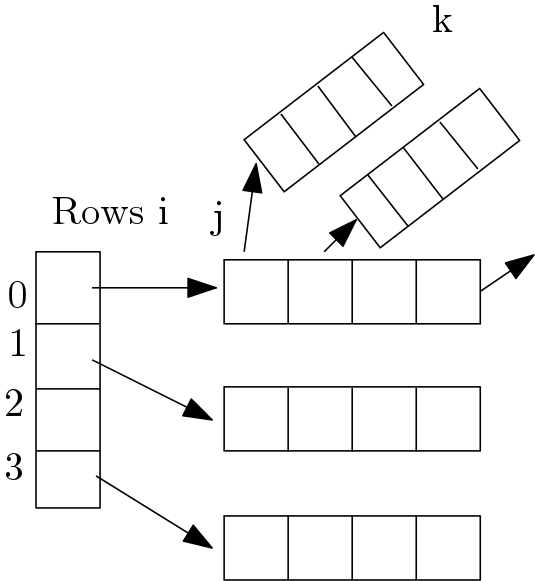
\includegraphics[width=0.3\linewidth]{LinkedList}
	\caption{Linked List Representation}
	\label{fig:linkedList}
\end{figure}

\textbf{Pros}
\begin{compactitem}
	\item Linked lists are fine if all of the data and processing is done in memory.
	\item Linked lists are extendible.
\end{compactitem}

\textbf{Cons}
\begin{compactitem}
	\item Linked lists are inappropriate for large files on the disk memory as linked lists can't be organized on the disk. As data warehousing works with big data the storage schema needs to be stored on the disk. 
\end{compactitem}

\subsection{Compressed Row/Column Storage}

 CRS representation makes use of three one-dimensional arrays to represent sparse 2D arrays. The \textbf{Value} array holds the non-zero elements from the 2D array, the \textbf{Column index} array holds the column indexes of each non-zero element, and the \textbf{Row pointer} array holds the offset value that starts a row \cite{wang:2014sar}.
 
 Using the example data given in Table \ref{tab:matrixmarket} and Figure \ref{fig:exampleMatrix} we give the CRS representation as shown in Table \ref{tab:compressed}.
 
  \begin{table}[H]
 	\caption{Compressed Row Storage Representation\label{tab:compressed}}
 	\begin{center}
 		\begin{tabular}{lllllllllllll}
 			\hline
 			{\textbf{Offset}} & 0 & 1 & 2 & 3 & 4 & 5 & 6 & ...& 14 & 15 & 16 & 17\\
 			\hline
 			{\textbf{Value}} & 5 & 7 & 42 & 30 & 9 & 30 & 70 & ...& 4 & 15 & 21 & 17 \\
 			{\textbf{Column index}} & 2 & 7 & 0 & 1 & 6 & 8 & 3 & ... & 1 & 1 & 2 & 17\\
 			{\textbf{Row Pointer}} & 0 & 2 & 6 & 8 & 10 & 12 & 13 & 15 & 16 & 17 & & \\
 			\hline
 		\end{tabular}
 	\end{center}
 \end{table}

\textbf{Pros}
\begin{compactitem}
	\item CRS and CCS have a wide usage - mainly with 2D arrays and image processing.
\end{compactitem}

\textbf{Cons}
\begin{compactitem}
	\item CRS and CCS are not appropriate representations of data stored on disk.
	\item CRS and CCS are not extendible - they require reorganising the entire array representation with the new additions by extending the bounds. Thus CRS and CCS are not appropriate in a dynamic environment when changes are happening rapidly.
	\item CRS and CCS representations are not appropriate for large arrays.
\end{compactitem}

\subsection{Bit Encoded Sparse Storage}
BESS uses a concatenation of the bit encoded representations of the indexes to generate a Bit Encoded Index (BEI). To improve storage for this method, a level of partitioning known as chunking is used. If $h_i, 0\leq i < k$ is the size of the chunk in each dimension, the number of chunks is $\prod_{i=0}^{k-1}[\frac{n_i}{h_i}]$. The storage required is $(\prod_{i=0}^{k-1}[\frac{n_i}{h_i}])*((c+ [\frac{\sum_{i=0}^{k-1}[\log h_i]}{wordsize}])N_{chunk})$. Only chunks that contain non-zero elements are stored.

For the example provided in Figure \ref{fig:exampleMatrix} if we were to divide the 2D array into 3x3 chunks we would get Figure \ref{fig:chunk} where the chunks breaks and discarded chunks are shown in blue.

 \begin{figure}[H]
	\centering
	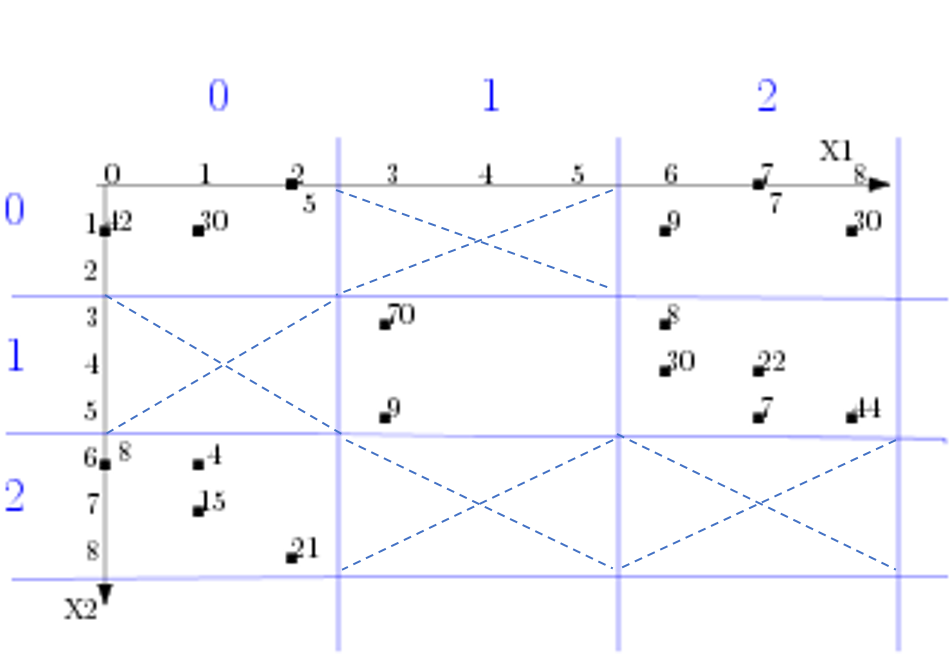
\includegraphics[width=0.7\linewidth]{chunked}
	\caption{BESS Chunking}
	\label{fig:chunk}
\end{figure}

The content from a non-empty chunk is stored as either a dense array or by using a sparse array method depending on the sparsity of the chunk.

\subsection{Comparisons of the Different Representations}

CRS and CCS are both only used for 2D arrays. In the work of Goil et al. \cite{goil:bess} it is clear that BESS out performs Offset-Value pair. In the work of Wang \cite{wang:2014sar} it is evident that although PTCS has a better storage ratio and xCRS/xCCS and BxCRS have faster element retrieval times, BESS has a faster construction time and a faster multi-dimensional aggregation time than all of the other storage schemes. 

BESS is a very simple and efficient multi-dimensional sparse array representation as it maps a multi-dimensional sparse array space to a one-dimensional array space, resulting in a bit encoded key index \cite{wang:2014sar}. A multi-dimensional sparse array data model using a BESS array representation scheme as well as a model using a CRS representation scheme will be analysed.

%%%%%%%%%%%%%%%%%%%%%%%%%%%%%%%%%%%%%%%%%%%%%%%%%%%%%%%%%%%%%%%%%%%%%%%%%%%%%%%%
\section{Extendible Multi-Dimensional Sparse Array Representation}

 By making use of chunking techniques on a BESS array representation scheme as well as a CRS array representation scheme. The proposed extendibility model can increase the dimensionality of the storage scheme by either increasing the density of the array or increasing the dimension of the indices or bounds of the array. When increasing a sparse array by density, the bounds and structure remain the same, new elements are slotted into a chunk where there was a free space. Extendibility of the bounds of the array is done by appending new chunks to the array. The two different extendibility techniques are displayed in red in Figure \ref{fig:examplemethod}.
 
  \begin{figure}[H]
 	\centering
 	\includegraphics[width=0.7\linewidth]{methodExampleCrossed2}
 	\caption{A Sparse 2D Array}
 	\label{fig:examplemethod}
 \end{figure}

\subsection{Multidimensional Sparse Array Blocks}
 In order to organise the chunks easily for reading and writing, a linear index of the array needs to be generated. Mapping for conventional arrays is done using row major order or column major order \cite{otoo:2013:ced}. Using column major order we have 
 \begin{equation}
 	\begin{split}
 		<i,j,k> & = C_0 C_1 C_2 \\
 		<i_0,j_0,k_0> = I & = i_0C_0 + j_0C_1 + k_0C_2
 	\end{split}
 \end{equation}
 where:
 \begin{align*}
 	C_0 & = X_1 \cdot X_2,\\
 	 C_1 & = X_2, \\
 	 C_2 & = 1
 \end{align*}
 
 An in memory index needs to be built into the blocks. As the indexing needs to be done in memory, multi-branching is not optimal, thus we focus on two way branching. Two important two way branches are the binary tree, and the PATRICIA Trie. Binary search trees are not balanced and can be skewed wasting storage space. PATRICIA stands for Practical Algorithm to Retrieve Information Coded In Alphanumeric \cite{morrison1968}. In PATRICIA Tries the skewness is compressed as it only compares bits that change the path and skips levels that are the same. If the chunk index values are stored and organised in a PATRICIA Trie we will avoid heavy sided trees and allow easy access to reading and writing of the array.
 
 \subsubsection{PATRICIA Trie representation of Blocks}
 Using the example in Figure \ref{fig:examplemethod} by labelling each chunk as A, B, C, D and E respectively and assigning their 2-bit row and 2-bit column indexing we obtain the bit indexing of the BESS chunks as shown in Table \ref{tab:index}. From this representation the PATRICIA Trie in Knuth representation is given in Figure \ref{fig:knuth}.
 
\begin{table}[H]
	\caption{Bit Indexing of BESS Chunks}\label{tab:index}
	\begin{center}
		\begin{tabular}{lll}
			\hline
			 \textbf{Linear Position} & \textbf{Bits} & \textbf{Chunk} \\
			\hline
			0 & 0000 & A \\
			2 & 0010 & B \\
			4 & 0100 & C \\
			5 & 0101 & D \\
			6 & 0110 & E \\
			\hline
		\end{tabular}
	\end{center}
\end{table}
 
 \begin{figure}[H]
 	\centering
 	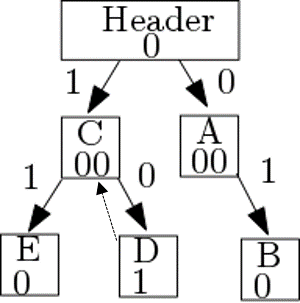
\includegraphics[width=0.25\linewidth]{knuth1}
 	\caption{Knuth representation of PATRICIA Trie indexing for the example in Figure \ref{fig:examplemethod}}
 	\label{fig:knuth}
 \end{figure}
 
 \section{Methodology for Accessing an Element from a Compressed Sparse Array}
 Suppose we have the compressed sparse array given in Figure \ref{fig:examplemethod} and we wish to find element 20 at position $<4,6>$. We will need to take the floor of the row and column indexes divided by the bounds of the matrix. I.e. we have $ \lfloor\frac{4}{3}\rfloor = 1$ and $\lfloor\frac{6}{3}\rfloor = 2$. Thus the block index is located at $<1,2>$ which has a linear address of $5$. We then use the PATRICIA Trie to locate the block. Once the block has been located, we use row major order to locate the element in the linear matrix within the block.
 
 \section{Project methodology}
 A sparse Big Data database will need to be sourced and stored. A BESS compression method as well as a CRS compression method will be applied to the database.
  
 The two algorithms for extension by appending and by inserting will need to be developed and implemented in software in order to determine which algorithm performs better. To assess the performance of the extendible multi-dimensional models, a measure of the storage efficiency and order of retrieval of queries shall be conducted using basic construction, low level retrieval and partial match query array operations.
 
 The two algorithms will be tested on a 2D array (both CRS and BESS), a 3D array(only BESS) and a 4D array(Only BESS) to asses their limitations on different dimensionalities. Figure \ref{fig:proposedmethod} shows the main steps in the proposed methodology of the project.
 
 \begin{figure}[H]
 	\centering
 	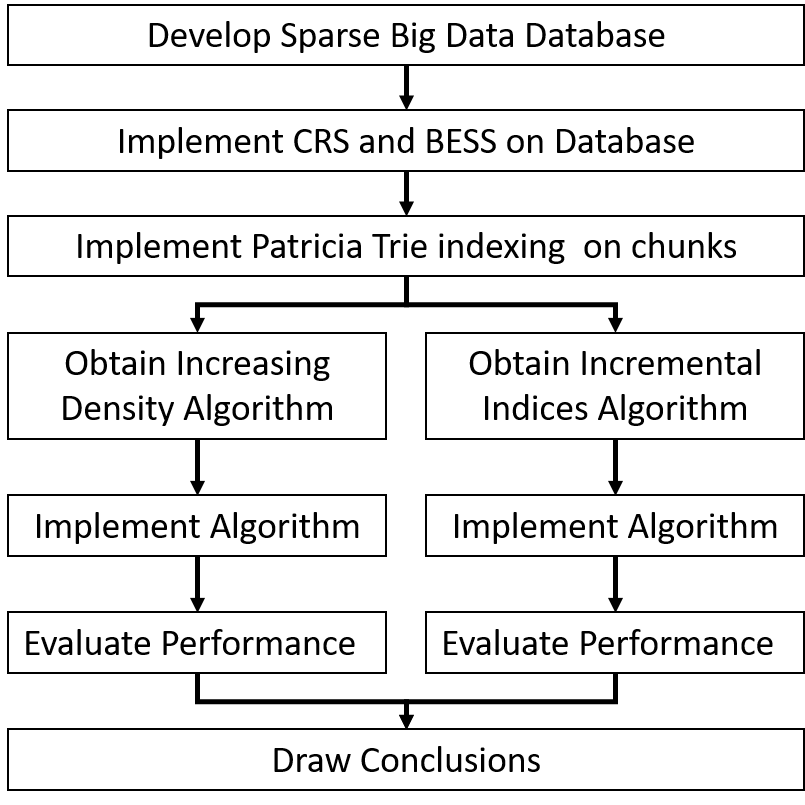
\includegraphics[width=0.7\linewidth]{proposedMethod2}
 	\caption{Proposed Methodology}
 	\label{fig:proposedmethod}
 \end{figure}
 
This representation can then be used in data warehousing where items are increased, stores can be acquired in new locations and new time frames can be added.
